\documentclass[a4paper]{article}

\usepackage{lmodern}

%% Language and font encodings
\usepackage[french]{babel}
\usepackage[utf8x]{inputenc}
\usepackage[T1]{fontenc}

%% Sets page size and margins
\usepackage[a4paper,top=3cm,bottom=3cm,left=2cm,right=2cm,marginparwidth=2cm]{geometry}

%% Useful packages
\usepackage{amsmath}
\usepackage{graphicx}
\usepackage[colorinlistoftodos]{todonotes}
\usepackage[colorlinks=true, allcolors=black]{hyperref}
\usepackage{fourier-orns}
\usepackage{titlesec}
\usepackage{fancyhdr}
\usepackage{fancyvrb}
\usepackage{enumitem}
\usepackage{float}
\usepackage{libertine}
\pagestyle{fancy} 
\setcounter{tocdepth}{5}

%% Tikz stuff
\usepackage{tikz}
\usetikzlibrary{calc, arrows}
\tikzstyle{incolore} = [rectangle, rounded corners, draw=black, minimum height=1cm, minimum width=3cm, text width=3cm, text centered]

\newcommand{\hsp}{\hspace{20pt}}
\newcommand{\HRule}{\rule{\linewidth}{0.5mm}}

% Défini la règle d'en-tête
\renewcommand{\headrulewidth}{1pt}
\fancyhead[C]{} 
\fancyhead[L]{}
\fancyhead[R]{\footnotesize{\leftmark}}

% Défini la règle de fond de page
\renewcommand{\footrulewidth}{1pt}
\fancyfoot[C]{} 
\fancyhead[L]{}
\fancyfoot[R]{\thepage}

\definecolor{Zgris}{rgb}{0.87,0.85,0.85}

\usepackage{eso-pic,graphicx}
\usepackage{xcolor}
\newcommand{\bgimg}[1]{
    \AddToShipoutPicture
    {
        \put(\LenToUnit{0 cm},\LenToUnit{0 cm})
        {
            \includegraphics[width=\paperwidth,height=\paperheight]{#1}
        }
    }
}

\begin{document}
\begin{titlepage}
    \begin{sffamily}
        \begin{center}
            \textnormal{}\\[6.5cm]
            \HRule \\[0.4cm]
            { \Huge \bfseries Synthèse\\ Physique appliqué\\ [0.4cm] }
            \HRule \\[3cm]
            \Large
            Premier Bloc\\
            Sécurité des systèmes\\
            Année académique 2019-2020\\[0.5cm]
            \emph{Rédigé par}\\
            \emph{Sénéchal Julien}
            \vfill
            {\large 06 Juin 2020}
        \end{center}
    \end{sffamily}
\end{titlepage}


\section{Unités du système international (SI)}
\begin{itemize}
    \item Courant électrique $\rightarrow$ A
    \item Température $\rightarrow$ K (Kelvin)
    \item Quantitée de matière $\rightarrow$ mol (mole)
    \item Intensité lumineuse $\rightarrow$ cd (Candela)
    \item Période (T)$\rightarrow$ s
    \item Fréquence $\rightarrow$ Hz (Hertz = $\frac{1}{s}$)
    \item Vitesse (v)$\rightarrow$ $\frac{m}{s}$
    \item Accelération (a)$\rightarrow$ $\frac{m}{s^{-2}}$
    \item Force (F)$\rightarrow$ N (newton = $masse (kg) \times acceleration $)
    \item Pression (P) $\rightarrow$ Pascal ($\frac{N}{m^2}$)
    \item Energie, travail, chaleur (E, W, Q) $\rightarrow$ J (joule = $N \times m$)
    \item Puissance (P) $\rightarrow$ W (watt = $\frac{joule}{s}$)
    \item Charge electrique $\rightarrow$ Q (Coulomb = $A \times s$)
    \item Tension (U) $\rightarrow$ V (Volt = $\frac{J}{s \times A}$ = $\frac{W}{A}$ = $\frac{J}{C}$)
    \item Résistance (R) $\rightarrow$ $\Omega$ (ohm = $\frac{V}{A}$)
    \item Puissance apparente (P) $\rightarrow$ $V \times A$
    \item Champ electrique (E) $\rightarrow$ $\frac{V}{m}$
    \item Champ magnetique (B) $\rightarrow$ T (tesla = $\frac{V \times s}{m^2}$)
    \item Masse volumique $\rho$ $\rightarrow$ $\frac{kg}{m^3}$
    \item Valume massique $\rightarrow$ $\frac{m^3}{kg}$
\end{itemize}
\scriptsize Heureusement qu'il n'y a que 26 lettres dans l'alphabet sinon on ne s'en serait pas sortit\dots
\normalsize

\begin{figure}[H]
    \centering
    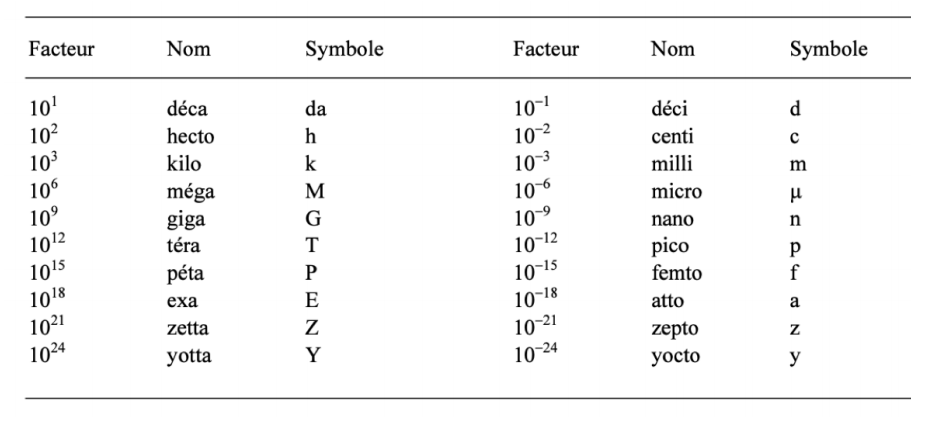
\includegraphics[width = 0.9 \textwidth]{images/1.PNG}
    \caption{Préfixes du système international}
\end{figure}

Quelques définitions :
\begin{itemize}
    \item Energie
    \begin{itemize}
        \item Ce qui permet d'agir (force en action). Capacité à produire un travail, modifier un état, etc...
    \end{itemize}
    \item Puissance
    \begin{itemize}
        \item Débit d'énergie 
        \item $Puissance = \frac{Energie}{temps}$
    \end{itemize}
    \item Watt-heure
    \begin{itemize}
        \item Le watt-heure est un débit de puissance (Energie)
    \end{itemize}
\end{itemize}

\section{Transfert Thermique}
\begin{itemize}
    \item Capacité thermique massique ($c_p$) :
        \begin{itemize}
            \item $\frac{J}{K \times kg}$
            \item Ordre de grandeur :
                \begin{itemize}
                    \item Energie pour augmenter la t° de 1 degré pour 1 litre d'eau est de 4185 Joules
                    \item $c_p$ eau = 4158 $\frac{J}{K \times kg}$
                    \item $c_p$ air = 1004 $\frac{J}{K \times kg}$
                    \item $c_p$ Aluminium = 897 $\frac{J}{K \times kg}$
                \end{itemize}
            \item Unitées :
                \begin{itemize}
                    \item Celsius
                    \item Farenheit
                    \item Kelvin
                    \item 0°C = 32°F = 273,15K
                    \item Convertir Celsius en Farenheit : $(x$°C$ \times 9/5) + 32 = y$°F
                    \item Convertir Farenheit en Celsius : $(y$°F$ − 32) \times 5/9 = x$°C
                    \item Convertir Celsius en Kelvin : $x$°C$ + 273,15 = y$°K
                \end{itemize}
        \end{itemize}
        \vspace{0.5cm}

    \item Conductivitée Thermique :
        \begin{itemize}
            \item $\lambda$ caractéristique a chaque matériaux
            \item Insique la quantitée de chaleur qui se propage par conduction thermique
            \item Unitées : $\frac{W}{m \times K}$
            \item Capacitée thermique massique : $\frac{J}{K \times kg}$
        \end{itemize}
        \vspace{0.5cm}
    \item Conduction :
        \begin{itemize}
            \item Transfert d'énergie sans déplacement de la matière
            \item Phénomène de diffusion
        \end{itemize}
    \item Convection :
        \begin{itemize}
            \item Déplacement de molécules qui permettent le déplacement de l'energie thermique
            \item Dans les fluides et sur les interfaces solides/fluides
        \end{itemize}
    \item Rayonnement :
        \begin{itemize}
            \item Rayonnement electromagnetique
            \item Souvent associé au rayonnement infrarouge
            \item Un corps émet un raonnement plus ou moins fort selon sa température
        \end{itemize}
        \vspace{0.5cm}
    \item Chauffe d'un processeur :
        \begin{itemize}
            \item $E = k \times f \times U^2$
            \begin{itemize}
                \item $f$ = fréquence du processeur (GHz)
                \item $U$ = tension d'alimentation (V)
                \item $k$ = constante de proportionnalitée (J/V)
            \end{itemize}
        \end{itemize}
\end{itemize}

\newpage
\section{Electricitée}
\textbf{Beaucoup de matière est abordée en Electronique appliquée Q1, et ne sera donc pas revu ici}\\[0.5cm]

Utilisation domestique :
\begin{itemize}
    \vspace{0.5cm}
    \item Disjoncteur
    \begin{itemize}
        \item Coupe le courant en cas de surcharge ou de court-circuit dans une installation
        \item Protection de l'installation électrique
        \item Sensibilitée de 10 à 25 A
        \item Un Disjoncteur pour chaque appareil (prise, four, lampe, lave-linge, etc...)
    \end{itemize}
    \vspace{0.5cm}
    \item Differentiel
    \begin{itemize}
        \item Coupe le courant en cas de détection d'une différence d'intensité du courant entre l'entrée et la sortie
        \item Protection des personnes
        \item Sensibilitée de 30 mA pour les salles d'eau et 300 mA pour les autres pièces
        \item Un Differentiel pour chaque pièce
    \end{itemize}
    \vspace{0.5cm}
    \item Prise de terre :
    \begin{itemize}
        \item Résistance max : 30 $\Omega$
        \item Protection contre les fuites de courant
    \end{itemize}
    \vspace{0.5cm}
    \item La masse :
    \begin{itemize}
        \item C'est un conducteur auxquel on va relier le circuit et qui servira de tension de référence. (Si celle-ci est reliée a la terre, alors elle est égale à 0V)
        \item Grâce a cette référence, nous pouvons être sûr que pour des signaux analogiques
        le 0 reste 0 et le 1 reste 1 et que la tension de passe donc pas dans des valeurs non permises.
    \end{itemize}
\end{itemize}


\vspace{0.5cm}
Effet de joule :
\begin{itemize}
    \item Echauffement lors du passage du courant 
    \item Résulte de la résistance aux charges électriques
    \item Dissipation d'énergie electrique sous forme de chaleur
\end{itemize}

\vspace{0.5cm}
Charges électrostatiques :
\begin{itemize}
    \item Accumulation de charges electriques à la surface d'un matériaux non conducteur
    \item Cause : Frottements de matériaux isolants (arrachement d'électrons)
    \item Conséquences : Dangereux pour le matériel électronique étant très sensible a ces charges (dégat de foudre)
    \item Protection contre ces charges : Mise à la terre
\end{itemize}

\vspace{0.5cm}
Electron volt :
\begin{itemize}
    \item $1 eV = 1,602 \times 10^{-19} J$
    \item Une charge de 1 électron accélérée par une différence de potentiel de 1 volt
    \item 1 Volt = 1 joule / 1 coulomb
\end{itemize}

\section{La puissance}
\begin{itemize}
    \item Dans un courant continu :
    \begin{itemize}
        \item $P = U \times I$
    \end{itemize}
    \item Dans un courant alternatif monophasé :
    \begin{itemize}
        \item $P = U_{eff} \times I_{eff}$
    \end{itemize}
    \item Dans un courant continu :
    \begin{itemize}
        \item $P = 3 \times U_{eff} \times I_{eff}$
    \end{itemize}
\end{itemize}
\vspace{0.5cm}
Différents types de puissances par induction:
\begin{itemize}
    \item Puissance active P (kW)
    \begin{itemize}
        \item Tous les appareils à induction qui fonctionnent sur les systèmes à courant alternatif convertissent l'énergie électrique fournie par
        l'alimentation en travail mécanique et/ou chaleur. Cette énergie est mesurée en kWh, et est appelée énergie "active".
        C’est la puissance réelle qui est transmise aux appareils.
    \end{itemize}
    \item Puissance réactive Q (kvar)
    \begin{itemize}
        \item Puissance nécessaire pour générer le champ magnétique (puissance perdue)
    \end{itemize}
    \item Puissance apparente S (kVA)
    \begin{itemize}
        \item Puissance apparente = Puissance active + puissance réactive
        \item Puissance apparente = $V_{eff} \times I_{eff}$
        \item La puissance apparente est la puissance totale pour qu'une installation fonctionne
        \item Le facteur de puissance $\phi$ :
        \begin{itemize}
            \item Rapport de puissance active P sur la puissance apparente S.
            \item On appelle aussi le "$cos\ \phi$" : "facteur de puissance"; il indique la qualité de la conception et de la gestion d'une installation électrique.*
            \item La valeur est comprise entre 1 et 0
        \end{itemize}
    \end{itemize}
\end{itemize}

\begin{figure}[H]
    \centering
    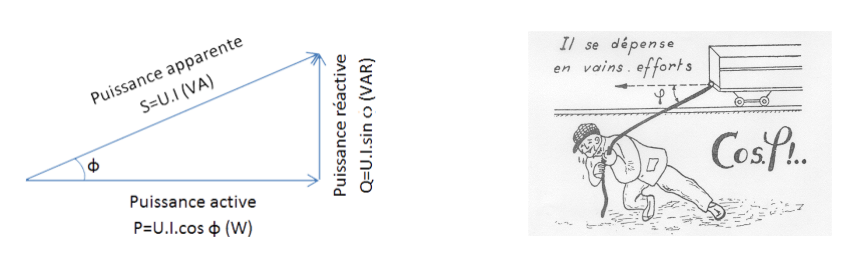
\includegraphics[width = 0.9 \textwidth]{images/2.PNG}
    \caption{Rapport des puissances}
\end{figure}

\newpage
\section{Electromagnetisme}
Magnétisme :
\begin{itemize}
    \item Ensemble de phénomènes physiques où les objets exercent des forces attractives/répulsives sur d'autres. 
\end{itemize}
\vspace{0.5cm}

Champ magnétique créé par un courant électrique continu
\begin{itemize}
    \item Tous les courants électriques créent des champs magnétiques H représenté en [A/m]
    \item $H = \frac{I}{2 \times \pi \times r}$
\end{itemize}

\vspace{0.5cm}

Notion de champ magnétique :
\begin{itemize}
    \item Le vecteur du champ créé par un courant se note H
    \item H = excitation magnétique = force magnétisante
    \item Théorème d'Ampère (théorème de la circulation) pour le bobinage :
    $$H = \frac{N\times I}{L}$$
    \begin{itemize}
        \item N = nombres de spires
        \item I = courant
        \item L = longueur du bobinage
    \end{itemize}
\end{itemize}
\vspace{0.5cm}

Notion d'induction magnétique :
\begin{itemize}
    \item $B = \mu \times H$
    \item $\mu = \mu_0 \times \mu_r$
    \item $\mu_0$ = perméabilitée du vide
    \item $\mu_r$ = perméabilitée relative
    \item $\mu$ = perméabilitée absolue
    \item Perméabilitée magnétique :
    \begin{itemize}
        \item Un matériau non magnétique dans un champ magnétique ne pertube pas le champ
        \item Un matériau magnétique dans un champ magnétique attire les lignes de forces vers lui plustôt que dans l'air
        \begin{itemize}
            \item Avant l'introduction d'un noyau ferromagnétique dans le champ : Flux magnétique = $\phi$
            \item Après l'introduction d'un noyau ferromagnétique dans le champ : $\phi' = \mu \times \phi$ et $\mu > 1$
        \end{itemize}
    \end{itemize}
\end{itemize}
\vspace{0.5cm}
L'induction magnétique B exprimé en Tesla ($= \frac{weber}{m^2} = \frac{kg}{A \times s^2}$): $$B = \frac{\phi}{S}$$
\vspace{0.5cm}
\section{Hystérésis}
\begin{figure}[H]
    \centering
    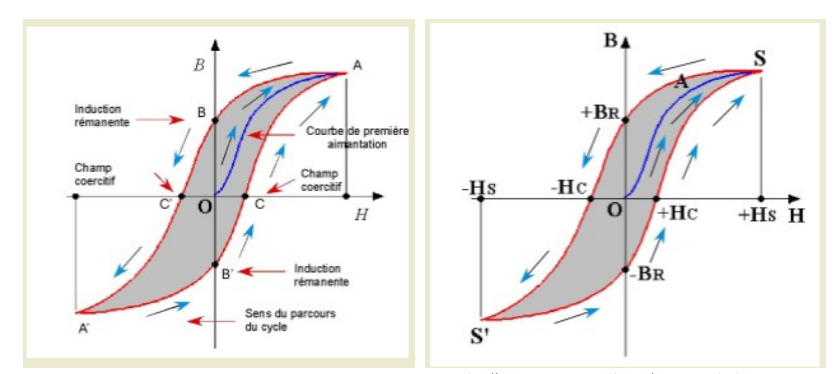
\includegraphics[width = 0.9 \textwidth]{images/3.PNG}
    \caption{Hystérésis}
\end{figure}
\begin{itemize}
    \item $B_R$ :
    \begin{itemize}
        \item Induction rémanente
        \item Induction qui subsiste dans l'échantillon après qu'on ait fait décroître H jusqu'à zéro.
    \end{itemize}
    \item $H_C$ :
    \begin{itemize}
        \item Champ coercitif
        \item Champ magnétique nécessaire pour annuler $B_R$
    \end{itemize}
    \item $B_R$ et $H_C$ sont spécifiques au matériau
    \item L'hystérésis est exprimée en $kg /m\times s^2$
    \item Son énergie : $kg \times m^2 / s^2$
\end{itemize}

\section{Force electromotrice}
La loi de Lenz : 
\begin{itemize}
    \item La force électromotrice induite
    tend à produire un courant qui s’oppose à la
    cause qui l’a produite.
    \item Pour bien comprendre cette loi, voir les 2 vidéos :\\ 
    https://www.youtube.com/watch?v=xOXwk6XtabE \\ 
    https://www.youtube.com/watch?v=XYirH7CzJys
\end{itemize}
La force de cette loi :
$$e = \frac{-d\times\phi}{d\times t}$$
\begin{center}
    e = La variation du flux sur une variation de temps\\
    Ou lors d'un cas particulier :
\end{center}
$$e = - B \times L \times v$$

\vspace{0.5cm}
La force electromotrice s'exprime en Volt :
\begin{itemize}
    \item $V = Tesla \times m \times m/s$
\end{itemize}

\section{RFID}
RFID = Identification par RadioFrequence
\begin{itemize}
    \item Permet d'identifier a distance des objets à l'arrêt ou en mouvement
    \item Permert d'échanger des données 
\end{itemize}
\vspace{0.5cm}
Constitution :
\begin{itemize}
    \item Un lecteur/scanner (antenne)
    \begin{itemize}
        \item Envoie une onde électromagnétique porteuse d'un signal vers les objets à identifier.
        \item Au retour du signal, le lecteur reçoit les informations de l'objet
    \end{itemize}
    \item Une étiquette
    \begin{itemize}
        \item Fixé sur l'objet
        \item Réagit à la reception du signal
        \item Comporte un microprocesseur avec une mémoire et connecté a une antenne.
    \end{itemize}
    \item Un ordinateur de stockage/traitement
    \begin{itemize}
        \item Va traiter les informations reçues par le lecteur
    \end{itemize}
\end{itemize}
\vspace{0.5cm}

2 modes d'interaction entre le lecteur et l'étiquette :
\begin{itemize}
    \item Couplage de nature inductive ou magnétique
    \item Couplage de nature radiative ou électromagnétique
\end{itemize}

\subsection{Couplage Magnétique}
A une distance maximale de l’ordre de la longueur d’onde, une source émet un
faisceau quasiment parallèle qui permet à la source d’entrer en
résonance inductive avec un récepteur.

\begin{itemize}
    \item Peu sensible aux perturbations
    \item Conception simple
    \item Peu coûteux
    \item Passif
    \item Portée limitée (max : 1,5m)
\end{itemize}

\subsection{Couplage radiatif}
En champ lointain, à une distance de la source
approximativement supérieure à la longueur
d’onde, le faisceau diverge pour donner
naissance à une onde sphérique localement
plane. L’étiquette se comporte alors
comme un véritable émetteur-récepteur radio et
nécessite en règle générale des solutions
actives. 

\begin{itemize}
    \item Permet une portée plus importante
    \item Débit de données plus important
    \item Antennes plus petites
    \item Système plus complexe
    \item Propagation des ondes plus difficile a prévoir
    \item Interferences difficiles a traiter
\end{itemize}

\subsection{Etiquette passive et active}

Etiquette active :
\begin{itemize}
    \item Possède une batterie
\end{itemize}
\vspace{0.5cm}
Etiquette passive :
\begin{itemize}
    \item Aucune autre source d’énergie que celle qu’elles reçoivent de la part du lecteur
\end{itemize}

\section{NFC}

NFC = Near Field Communication
\begin{itemize}
    \item Permet la reconnaissance mutuelle à très courte distance (0 à 20cm)
    \item But : Mettre en relation 2 dispositifs électroniques qui pourront s'échanger des informations
\end{itemize}



































\end{document}